\documentclass[aspectratio=1610]{beamer}

\usepackage[utf8]{inputenc}
\usepackage{inconsolata}
\usepackage[scaled]{beramono}
\usepackage[T1]{fontenc}
\usepackage{amsmath}
\usepackage{tikz}
%\usepackage{tikzlings}
%\usepackage{tikzpeople}
\usepackage{pgfplots}
\usepackage{changepage}
\usepackage{environ}
\usepackage{listings}
\usepackage{mathabx}
\usepackage{csquotes}
\usepackage{savesym}
\savesymbol{checkmark}
\usepackage{dingbat}
\usetikzlibrary{positioning}
\usetikzlibrary{shapes.arrows}
\usetikzlibrary{matrix}
\usetikzlibrary{calc}
\usetikzlibrary{decorations.pathmorphing}

\usetheme{metropolis}
\setbeamercolor{alerted text}{fg=teal, bg=white}
\setbeamercolor{normal text}{bg=white}

\title{Bioinformatics Preparatory Course}
\subtitle{Basic Unix}
\author{Léon Kuchenbecker and Sam Wein}
\date{October 21, 2020}

\newcommand\sepsym{\raisebox{.1em}{\tiny$\blacksquare$} }
\newcommand\curtitle{}

%\lstset{
%                basicstyle=\color{white}\ttfamily,
%                keywordstyle=\color{magenta}\ttfamily,
%                stringstyle=\color{orange}\ttfamily,
%                commentstyle=\color{blue}\ttfamily,
%                morecomment=[l][\color{blue}]{\#},
%                escapeinside={(*}{*)},
%                belowskip=0mm,
%                aboveskip=0mm,
%}



\tikzset{
    codebox/.style={
        line width=0mm,
        text width=\linewidth-17.1pt,
        fill=black,
        %rounded corners=.5mm,
        inner xsep=3mm,
        inner ysep=0mm,
    },
}

\newcommand{\footercomment}[1]{
    \begin{tikzpicture}[overlay, remember picture]
        \node [anchor=west, font=\scriptsize] at ($(current page.south west)+(1.5mm,4.70mm)$) {#1};
    \end{tikzpicture}
}

%%%%%%%%%%%%%%%%%%%%%%%%%%%%%%%%%%%%%%%%%%%%%%%%%%%%%%%%%%%%%%%%%%%%%%%%%%%%%%%%%%%%%%%%%%%%%%%%%%%%

\colorlet{keyboard}{gray}
\colorlet{stdout}{teal}
\colorlet{stderr}{orange}
\makeatletter

\newenvironment{shells}[1]{
    \begin{tikzpicture}[codebox/.append style={text width=#1-18pt}]
        \coordinate (code);
}{
    \end{tikzpicture}
}
\lstnewenvironment{shellout}[1][keyboard]{%
    \lstset{%
        basicstyle=\color{white}\ttfamily\bfseries\small,
        escapeinside={(*}{*)},
        belowskip=0mm,
        aboveskip=0mm,
    }%
    \node[codebox, below=0mm of code] (code) \bgroup
}%
{%
    \egroup;
    \draw [line width=2mm,#1] ($(code.north east)-(1mm,0mm)$) -- ($(code.south east)-(1mm,0mm)$)
        ($(code.north west)+(1mm,0mm)$) -- ($(code.south west)+(1mm,0mm)$);
}
\lstnewenvironment{shelloutsmall}[1][keyboard]{%
    \lstset{%
        basicstyle=\color{white}\ttfamily\bfseries\scriptsize,
        escapeinside={(*}{*)},
        belowskip=0mm,
        aboveskip=0mm,
    }%
    \node[codebox, below=0mm of code] (code) \bgroup
}%
{%
    \egroup;
    \draw [line width=2mm,#1] ($(code.north east)-(1mm,0mm)$) -- ($(code.south east)-(1mm,0mm)$)
        ($(code.north west)+(1mm,0mm)$) -- ($(code.south west)+(1mm,0mm)$);
}

\makeatother

\newcommand\command[1]{\alert{\textbf{\texttt{#1}}}}

\begin{document}

%%%%%%%%%%%%%%%%%%%%%%%%%%%%%%%%%%%%%%%%%%%%%%%%%%%%%%%%%%%%%%%%%%%%%%%%%%%%%%%%%%%%%%%%%%%%%%%%%%%%

\begin{frame}
    \titlepage
\end{frame}


%%%%%%%%%%%%%%%%%%%%%%%%%%%%%%%%%%%%%%%%%%%%%%%%%%%%%%%%%%%%%%%%%%%%%%%%%%%%%%%%%%%%%%%%%%%%%%%%%%%%

\begin{frame}[c]{Why bother with the shell?}
    \begin{itemize}[<+->]\setlength\itemsep{1em}
        \item The shell is extremely powerful

            \begin{itemize}[<.->]
                \item Searching, organizing, transferring large numbers of files
                \item Exploring and manipulating plain text files
                \item Can be programmed
            \end{itemize}

        \item The shell can be executed remotely

            \begin{itemize}[<.->]
                \item SSH (secure shell) interface to access a Unix-like system remotely
                \item Standard to interact with larger computer infrastructures (e.g. a compute
                    server or cluster)
            \end{itemize}

        \item The majority of bioinformatics tools have a CLI
            \begin{itemize}[<.->]
                \item We work with a high number of large files
                \item Crunching that data requires high compute power $\Rightarrow$ compute server,
                    cluster
                \item Most file formats established in Bioinformatics are plain text
            \end{itemize}
    \end{itemize}
\end{frame}

%%%%%%%%%%%%%%%%%%%%%%%%%%%%%%%%%%%%%%%%%%%%%%%%%%%%%%%%%%%%%%%%%%%%%%%%%%%%%%%%%%%%%%%%%%%%%%%%%%%%

\begin{frame}[c,fragile]{Basic Usage}
    \begin{itemize}
        \item Enter a command and press the Return ($\dlsh$) key
            \begin{shells}{\linewidth}
                \begin{shellout}
(*$\mathdollar$*) ls (*$\dlsh$*)
                \end{shellout}
                \begin{shellout}[stdout]
Desktop   Documents   Exercise
                \end{shellout}
            \end{shells}
        \item To get help on how to use a particular command, try
            \begin{shells}{\linewidth}
                \begin{shellout}
(*$\mathdollar$*) ls --help (*$\dlsh$*)
(*$\mathdollar$*) man ls (*$\dlsh$*)
                \end{shellout}
            \end{shells}
        \item The basic command syntax often follows this structure:
            \begin{shells}{\linewidth}
                \begin{shellout}
COMMAND [OPTIONAL SWITCHES] [MANDATORY ARGUMENTS] 
                \end{shellout}
            \end{shells}
    \end{itemize}
\end{frame}

%%%%%%%%%%%%%%%%%%%%%%%%%%%%%%%%%%%%%%%%%%%%%%%%%%%%%%%%%%%%%%%%%%%%%%%%%%%%%%%%%%%%%%%%%%%%%%%%%%%%

\begin{frame}[c,fragile]{Basic Usage}
    \begin{itemize}[<+->]
        \item Often there are long (\verb|--|) and short (\verb|-|) versions of switches
            \begin{shells}{\linewidth}
                \begin{shellout}
(*$\mathdollar$*) ls (*$\dlsh$*)
                \end{shellout}
                \begin{shellout}[stdout]
Desktop   Documents   Exercise
                \end{shellout}
                \begin{shellout}
(*$\mathdollar$*) ls -r (*$\dlsh$*)
                \end{shellout}
                \begin{shellout}[stdout]
Exercise    Documents    Desktop
                \end{shellout}
                \begin{shellout}
(*$\mathdollar$*) ls --reverse (*$\dlsh$*)
                \end{shellout}
                \begin{shellout}[stdout]
Exercise    Documents    Desktop
                \end{shellout}
            \end{shells}
        \item Multiple switches can be specified together
            \begin{shells}{\linewidth}
                \begin{shellout}
(*$\mathdollar$*) ls -F -r (*$\dlsh$*)
                \end{shellout}
                \begin{shellout}[stdout]
Exercise/  Documents/  Desktop/
                \end{shellout}
                \begin{shellout}
(*$\mathdollar$*) ls -Fr (*$\dlsh$*)
                \end{shellout}
                \begin{shellout}[stdout]
Exercise/  Documents/  Desktop/
                \end{shellout}
            \end{shells}
    \end{itemize}
\end{frame}

%%%%%%%%%%%%%%%%%%%%%%%%%%%%%%%%%%%%%%%%%%%%%%%%%%%%%%%%%%%%%%%%%%%%%%%%%%%%%%%%%%%%%%%%%%%%%%%%%%%%
\renewcommand\curtitle{File systems}
%%%%%%%%%%%%%%%%%%%%%%%%%%%%%%%%%%%%%%%%%%%%%%%%%%%%%%%%%%%%%%%%%%%%%%%%%%%%%%%%%%%%%%%%%%%%%%%%%%%%

\begin{frame}[c]
    \Huge \curtitle
\end{frame}

\begin{frame}[c]{\curtitle}
    A typical computer \alert{file system} is structured like a \alert{tree}

    \medskip\centering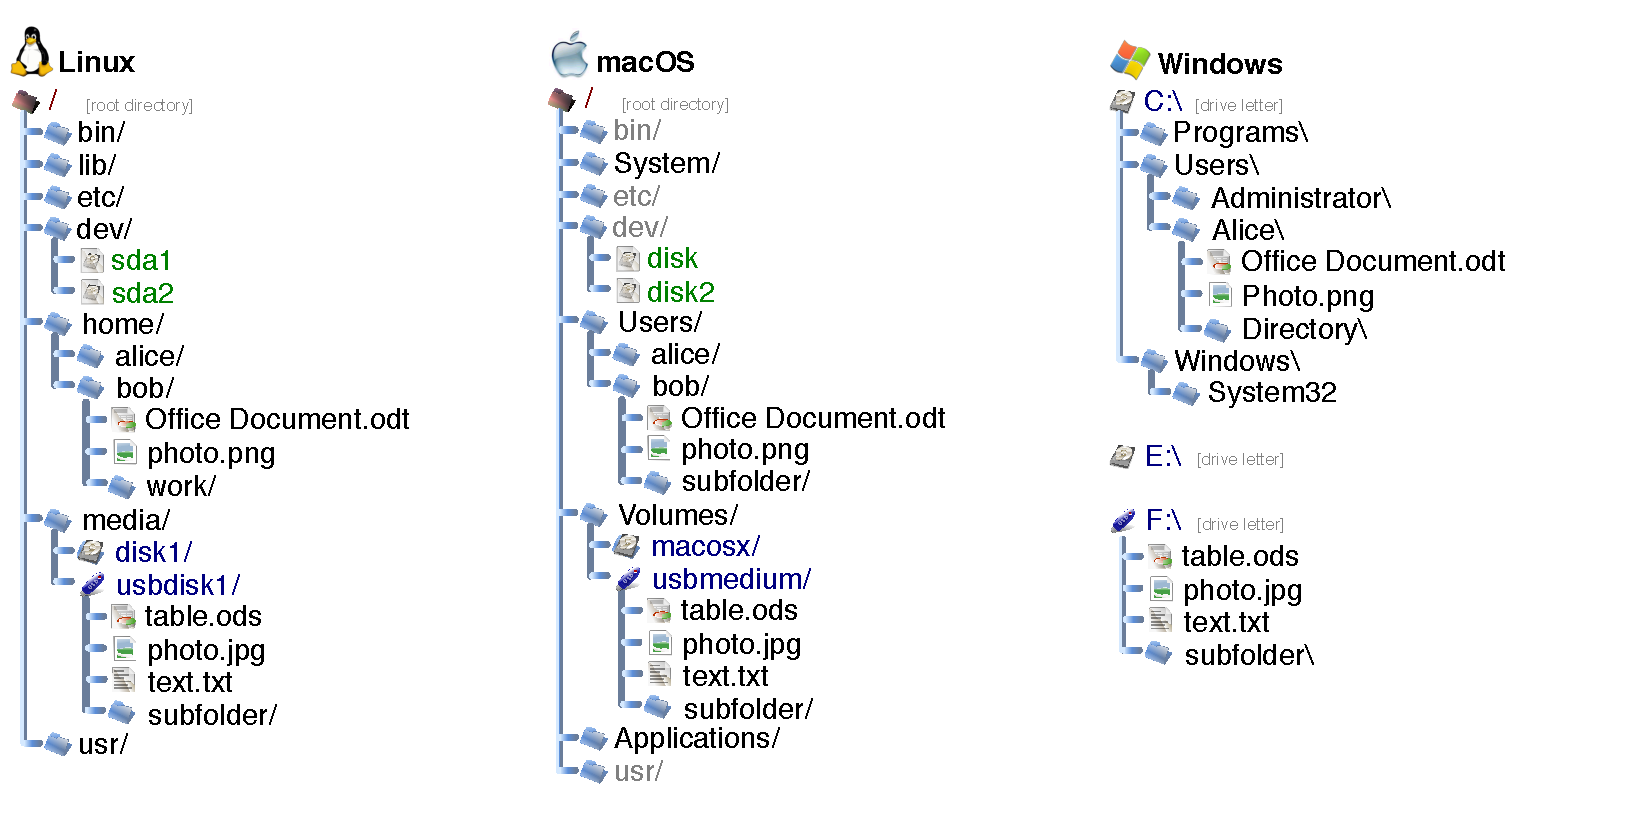
\includegraphics[width=\linewidth]{filesystem.pdf}
\end{frame}

%%%%%%%%%%%%%%%%%%%%%%%%%%%%%%%%%%%%%%%%%%%%%%%%%%%%%%%%%%%%%%%%%%%%%%%%%%%%%%%%%%%%%%%%%%%%%%%%%%%%

\begin{frame}[c]{\curtitle}
    \begin{itemize}[<+->]\setlength\itemsep{1em}
        \item Every running computer program, i.e. every process, including the \alert{shell}, refers to one directory
            inside the file system tree as its \alert{working directory}.
        \item When using the \alert{shell}, one often says \enquote{I am in the directory xzy}.
        \item The \alert{working directory} is not static, it can be changed throughout the runtime of a process.
    \end{itemize}
\end{frame}

\begin{frame}[c]{\curtitle}
    \begin{adjustwidth}{-2em}{-2em}
        \begin{columns}
            \begin{column}{0.32\textwidth}
                \begin{tikzpicture}
                    \node [inner sep=0mm] (pic) {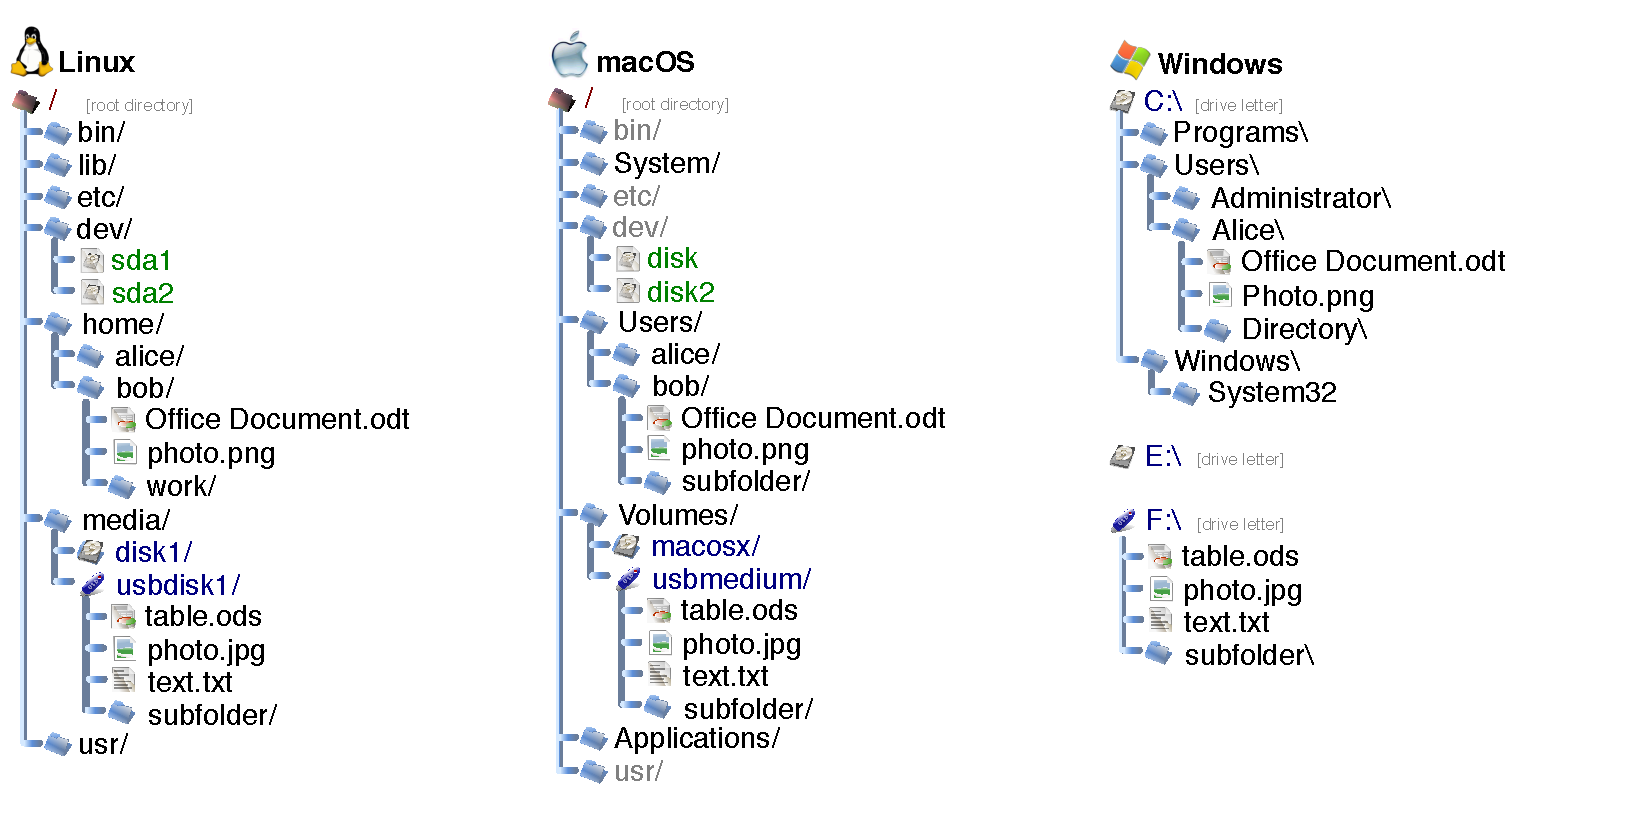
\includegraphics[height=\textheight, trim=0mm 0mm 208mm 0mm, clip]{filesystem.pdf}};
                    \visible<2->{
                    \node [fill=red,draw, circle, inner sep=0mm, text width=2.5mm, red] (root) at ($(pic.north west)+(3mm,-11.2mm)$) {};
                    \node [fill=red,draw, circle, inner sep=0mm, text width=2.5mm, red] (home) at ($(pic.north west)+(6.5mm,-35.4mm)$) {};
                    \node [fill=red,draw, circle, inner sep=0mm, text width=2.5mm, red] (bob) at ($(pic.north west)+(10mm,-42.3mm)$) {};
                    \node [rounded corners, draw=red, text width=20mm, minimum height=4mm, inner
                        sep=0mm, line width=1pt] (file) at ($(pic.north west)+(22mm, -49.5mm)$) {};
                        \draw [line width=2pt, red] (root) |- (home) |- (bob) |- (file);
                    }
                \end{tikzpicture}
            \end{column}
            \begin{column}{0.70\textwidth}
                \begin{itemize}[<+->]\setlength\itemsep{1em}
                    \item Every file or directory in the file system can be described by a \alert{path}
                    \item \alert{Absolute paths} start in the root directory, for example

                        \medskip\texttt{/home/bob/photo.png}
                    \item \alert{Relative paths} start in the current working directory, for example

                        \medskip\texttt{./bob/photo.png}

                        \medskip given that the current working directory is \texttt{/home}.
                    \item Every character sequence that does not start with a slash \alert{\texttt{/}} character
                        is interpreted as a relative path.
                \end{itemize}
            \end{column}
        \end{columns}
    \end{adjustwidth}
\end{frame}

%%%%%%%%%%%%%%%%%%%%%%%%%%%%%%%%%%%%%%%%%%%%%%%%%%%%%%%%%%%%%%%%%%%%%%%%%%%%%%%%%%%%%%%%%%%%%%%%%%%%
\renewcommand\curtitle{Working with the file system}
%%%%%%%%%%%%%%%%%%%%%%%%%%%%%%%%%%%%%%%%%%%%%%%%%%%%%%%%%%%%%%%%%%%%%%%%%%%%%%%%%%%%%%%%%%%%%%%%%%%%


\begin{frame}[c]{\curtitle}
    \begin{itemize}[<+->]
        \setlength\itemsep{1em}
        \item \command{pwd} \textbf{- print working directory} 

            Prints the current working directory
        \item \command{ls} \textbf{- list} 

            Displays the contents of folders (directories)
            \begin{itemize}[<.->]
                \item \alert{\texttt{ls -l}} show details
                \item \alert{\texttt{ls -lh}} human readable file sizes
                \item \alert{\texttt{ls -l}} show hidden files and folders
            \end{itemize}
        \item \command{cd} \textbf{- change directory} 

            Changes the current working directory
    \end{itemize}
\end{frame}

%%%%%%%%%%%%%%%%%%%%%%%%%%%%%%%%%%%%%%%%%%%%%%%%%%%%%%%%%%%%%%%%%%%%%%%%%%%%%%%%%%%%%%%%%%%%%%%%%%%%


\begin{frame}[c]{\curtitle}
    \begin{itemize}[<+->]
        \setlength\itemsep{1em}
        \item \command{mkdir <path>} \textbf{- make directory} 

            Creates a new directory
        \item \command{cp <source path> <destination path>} \textbf{- copy} 

            Copies files and folders. \textcolor{red}{\textbf{Overwriting targets cannot be
            undone!}}
            \begin{itemize}[<.->]
                \item \command{cp -r} - recursive mode

                    Required to copy directories with their contents.
            \end{itemize}
        \item \command{mv <source path> <destination path>} \textbf{- move} 

            Move files and folders \textcolor{red}{\textbf{Overwriting targets cannot be undone!}}
        \item \command{rmdir <path>} \textbf{- remove directory} 

            Removes directories, but only if they are empty. Safe to use.
    \end{itemize}
\end{frame}

%%%%%%%%%%%%%%%%%%%%%%%%%%%%%%%%%%%%%%%%%%%%%%%%%%%%%%%%%%%%%%%%%%%%%%%%%%%%%%%%%%%%%%%%%%%%%%%%%%%%

\begin{frame}[c]{\curtitle}
    \begin{itemize}[<+->]
        \setlength\itemsep{1em}
        \item \command{rm <path>} \textbf{- remove} 

            Remove files and folders. \textcolor{red}{\textbf{Removing cannot be undone!}}
            \begin{itemize}[<.->]
                \item \command{cp -r} - recursive mode

                    Required to remove directories with their contents.
            \end{itemize}
    \end{itemize}
\end{frame}

%%%%%%%%%%%%%%%%%%%%%%%%%%%%%%%%%%%%%%%%%%%%%%%%%%%%%%%%%%%%%%%%%%%%%%%%%%%%%%%%%%%%%%%%%%%%%%%%%%%%

\begin{frame}[c]
    \Huge Getting started with plain text files
\end{frame}

\renewcommand\curtitle{Inspecting plain text files}

\begin{frame}[c]{\curtitle}
    \begin{itemize}[<+->]
        \setlength\itemsep{1em}
        \item \command{more <path>}

            Page through text one page at a time
        \item \command{less <path>} \textbf{- the opposite of more}

            More powerful than more, bidirectional, provides searching
        \item \command{cat <path> [<path> ...]} \textbf{- concatenate}

            Concatenates input files and prints them to the standard output (more on that later).
    \end{itemize}
\end{frame}

%%%%%%%%%%%%%%%%%%%%%%%%%%%%%%%%%%%%%%%%%%%%%%%%%%%%%%%%%%%%%%%%%%%%%%%%%%%%%%%%%%%%%%%%%%%%%%%%%%%%

\begin{frame}[c]{\curtitle}
    \begin{itemize}[<+->]
        \setlength\itemsep{1em}
        \item \command{head <path>}

            Output the first $n$ lines of a plain text file.
        \item \command{tail <path>}

            Output the last $n$ lines of a plain text file.
            \begin{itemize}[<.->]
                \item \command{tail -f} - follow

                    Keeps printing new lines as the file grows.
            \end{itemize}

    \end{itemize}
\end{frame}

%%%%%%%%%%%%%%%%%%%%%%%%%%%%%%%%%%%%%%%%%%%%%%%%%%%%%%%%%%%%%%%%%%%%%%%%%%%%%%%%%%%%%%%%%%%%%%%%%%%%

\renewcommand\curtitle{Creating and editing plain text files}

\begin{frame}[c]{\curtitle}
    \begin{itemize}[<+->]
        \setlength\itemsep{1em}
        \item A \alert{text editor} is a program used to edit plain text files
        \item Well known graphical editors are \alert{Notepad} on Microsoft Windows and
            \alert{TextEdit} on Apple macOS
        \item \alert{Nano} is a text editor that does not require a graphical user interface but
            works on the command line
    \end{itemize}
\end{frame}

%%%%%%%%%%%%%%%%%%%%%%%%%%%%%%%%%%%%%%%%%%%%%%%%%%%%%%%%%%%%%%%%%%%%%%%%%%%%%%%%%%%%%%%%%%%%%%%%%%%%

\begin{frame}[c]{\curtitle}
    \begin{itemize}[<+->]
        \setlength\itemsep{1em}
    \item \command{nano <path>}

        Opens the file specified by path. Can be used on non-existing paths to create
        new files.
    \item \command{CTRL-O}

        Saves the current file
    \item \command{CTRL-X}

        Exits nano
\end{itemize}
\end{frame}

%%%%%%%%%%%%%%%%%%%%%%%%%%%%%%%%%%%%%%%%%%%%%%%%%%%%%%%%%%%%%%%%%%%%%%%%%%%%%%%%%%%%%%%%%%%%%%%%%%%%

\renewcommand\curtitle{Keyboard shortcuts}

\begin{frame}[c]{\curtitle}
    \begin{itemize}
        \item \command{TAB}

            Autocomplete the command line
        \item \command{TAB - TAB}

            Show possible completions if not unique
        \item \command{ALT-b} and \command{ALT-f}

            Move one word backward (or forward) in the current command line
        \item \command{Pos1} or \command{Home}

            Move to the beginning of the current command line
        \item \command{End}

            Move to the end of the current command line
    \end{itemize}
\end{frame}

%%%%%%%%%%%%%%%%%%%%%%%%%%%%%%%%%%%%%%%%%%%%%%%%%%%%%%%%%%%%%%%%%%%%%%%%%%%%%%%%%%%%%%%%%%%%%%%%%%%%

\begin{frame}[c]{\curtitle}
    \centering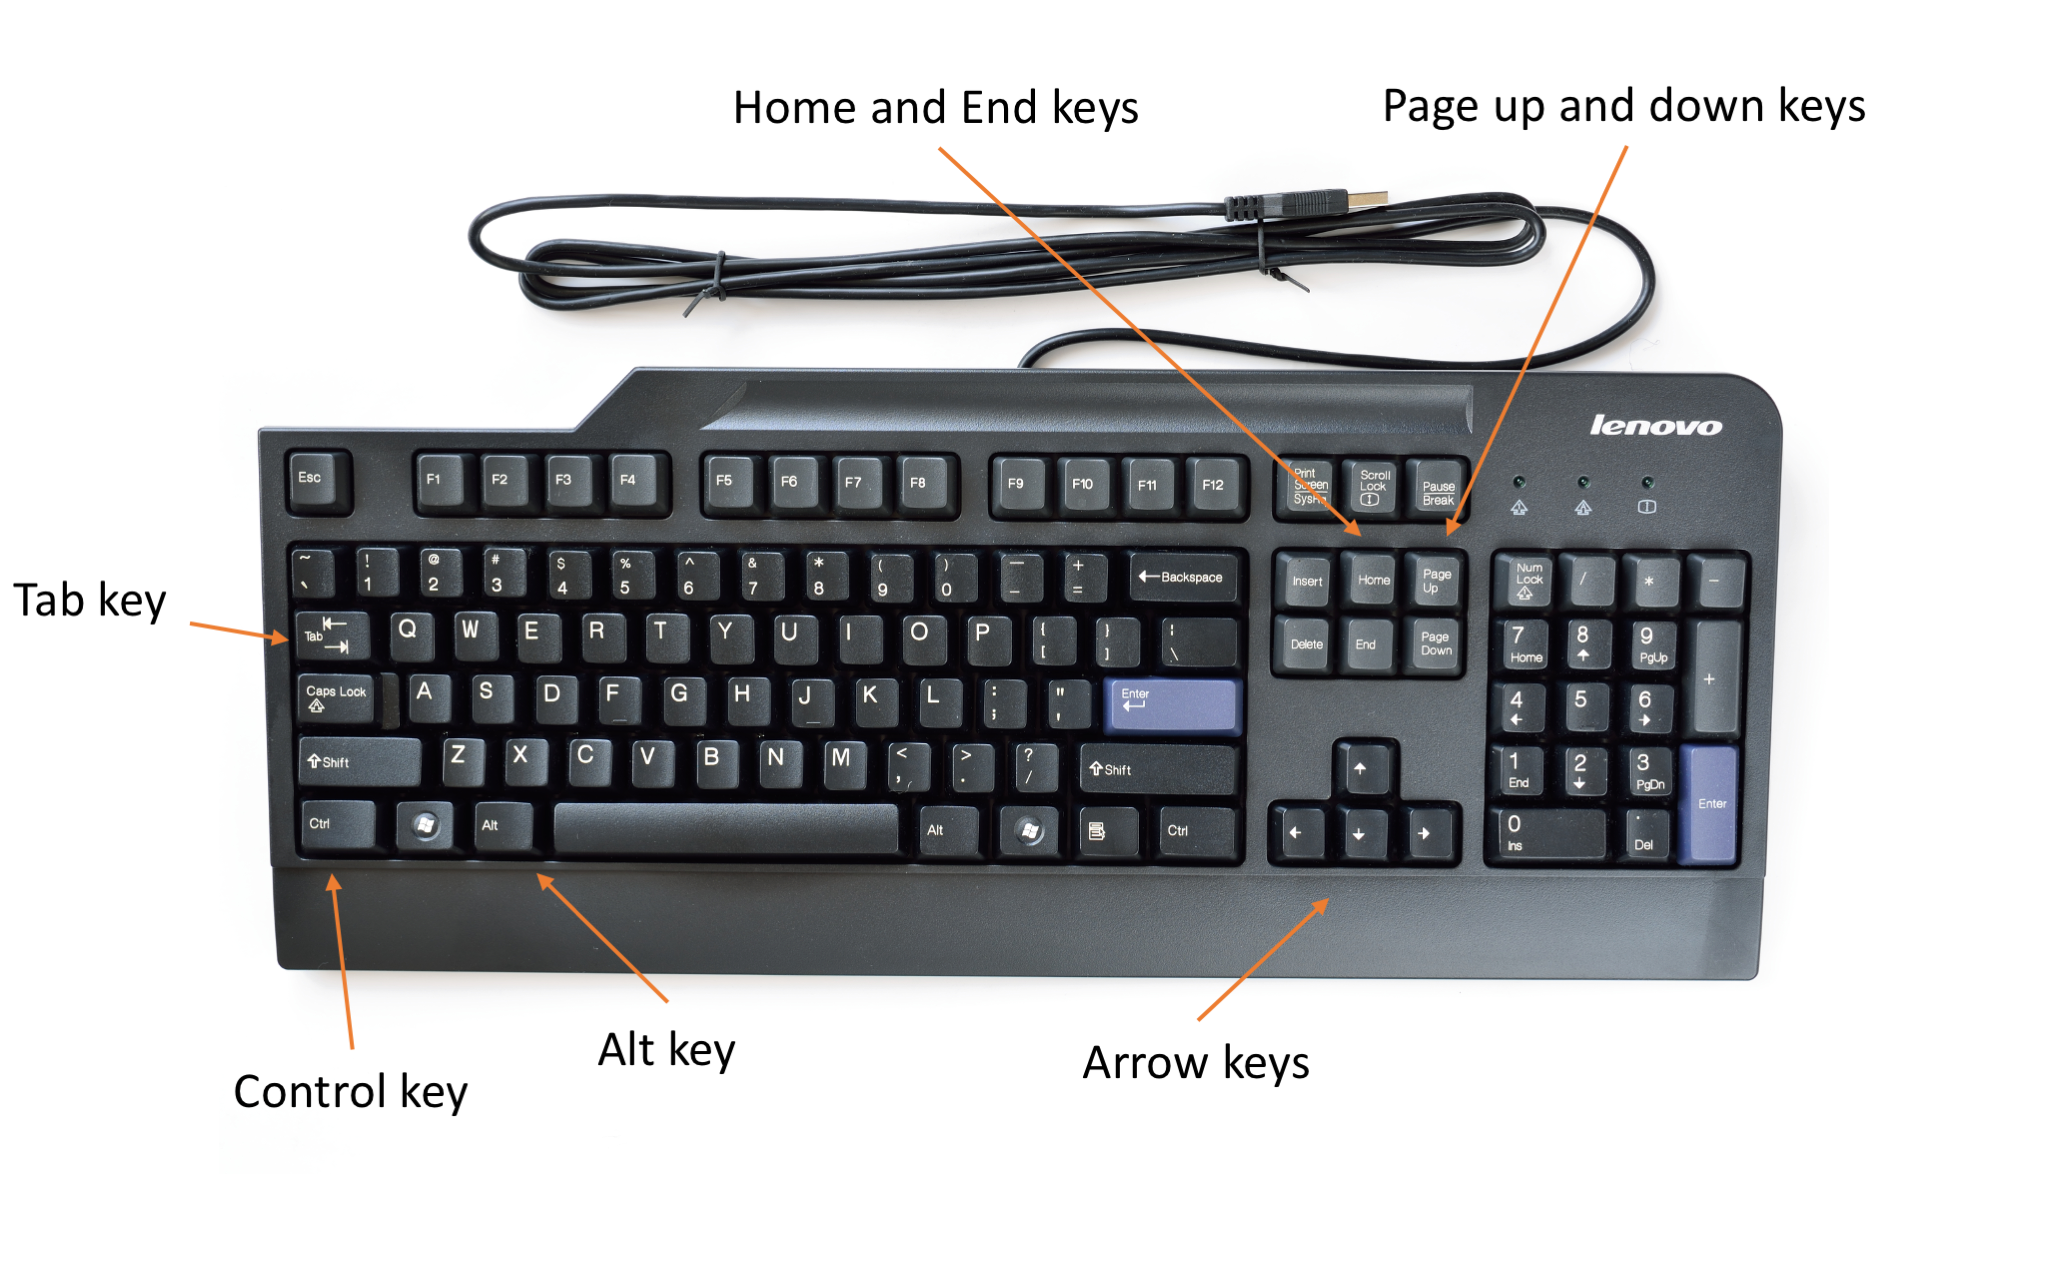
\includegraphics[width=\linewidth]{keyboard.png}
\end{frame}

%%%%%%%%%%%%%%%%%%%%%%%%%%%%%%%%%%%%%%%%%%%%%%%%%%%%%%%%%%%%%%%%%%%%%%%%%%%%%%%%%%%%%%%%%%%%%%%%%%%%

\begin{frame}[c]{\curtitle}
    \begin{itemize}
        \item \command{Arrow Up}

            Browse the shell history backward in time
        \item \command{Arrow Down}

            Browse the shell history forward in time
        \item \command{CTRL-R}

            Search the shell history backward in time
        \item \command{CTRL-C}

            Interrupt the current program.
    \end{itemize}
\end{frame}

%%%%%%%%%%%%%%%%%%%%%%%%%%%%%%%%%%%%%%%%%%%%%%%%%%%%%%%%%%%%%%%%%%%%%%%%%%%%%%%%%%%%%%%%%%%%%%%%%%%%
\renewcommand\curtitle{Process streams}
%%%%%%%%%%%%%%%%%%%%%%%%%%%%%%%%%%%%%%%%%%%%%%%%%%%%%%%%%%%%%%%%%%%%%%%%%%%%%%%%%%%%%%%%%%%%%%%%%%%%

\begin{frame}[c]
    \Huge \curtitle
\end{frame}

%%%%%%%%%%%%%%%%%%%%%%%%%%%%%%%%%%%%%%%%%%%%%%%%%%%%%%%%%%%%%%%%%%%%%%%%%%%%%%%%%%%%%%%%%%%%%%%%%%%%

\begin{frame}[c]{\curtitle}
    \begin{itemize}
        \item Every \alert{process} has three input / output streams
            \begin{itemize}
                \item Standard input (stdin)
                \item Standard output (stdout)
                \item Standard error (stderr)
            \end{itemize}
    \end{itemize}

    \pause
    \centering
    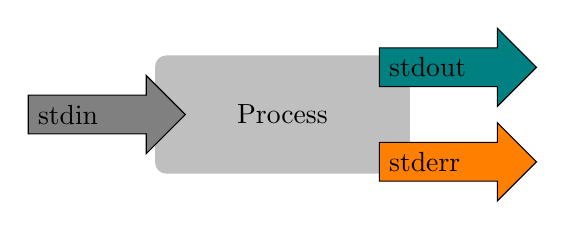
\begin{tikzpicture}
        \node [rounded corners, fill=gray!50, minimum height=15mm, text width=30mm, align=center]
            (proc)
            {Process};
        \node [draw, single arrow, fill=gray, anchor=east, text width=15mm] at ($(proc.west)+(4mm,0)$) {stdin};
        \node [draw, single arrow, fill=teal, anchor=west, text width=15mm] at ($(proc.east)+(-4mm,6mm)$) {stdout};
        \node [draw, single arrow, fill=orange, anchor=west, text width=15mm] at ($(proc.east)+(-4mm,-6mm)$) {stderr};
    \end{tikzpicture}
    \pause
    \begin{itemize}
        \item We have so far \alert{only worked with stdout}.
    \end{itemize}
\end{frame}

%%%%%%%%%%%%%%%%%%%%%%%%%%%%%%%%%%%%%%%%%%%%%%%%%%%%%%%%%%%%%%%%%%%%%%%%%%%%%%%%%%%%%%%%%%%%%%%%%%%%

\begin{frame}[fragile, c]{\curtitle}
    \begin{itemize}[<+->]
        \setlength\itemsep{1em}
        \item Normally, we cannot see the differente between \alert{stdout} and \textcolor{orange}{stderr}

        \item This output is produced on \alert{stdout}
            \begin{shells}{\linewidth}
                \begin{shellout}
(*$\mathdollar$*) ls -l Exercise/data (*$\dlsh$*)
                \end{shellout}
                \begin{shellout}[stdout]
total 13960
-rw-r--r-- 1 vorkurs vorkurs 14293917 Mar 27  2018 clinvar_20180225.vcf.gz
                \end{shellout}
            \end{shells}
        \item This output is produced on \textcolor{orange}{stderr}
            \begin{shells}{\linewidth}
                \begin{shellout}
(*$\mathdollar$*) ls -l doesnt.exist (*$\dlsh$*)
                \end{shellout}
                \begin{shellout}[stderr]
ls: cannot access 'doesnt.exist': No such file or directory
                \end{shellout}
            \end{shells}
    \end{itemize}
\end{frame}

%%%%%%%%%%%%%%%%%%%%%%%%%%%%%%%%%%%%%%%%%%%%%%%%%%%%%%%%%%%%%%%%%%%%%%%%%%%%%%%%%%%%%%%%%%%%%%%%%%%%

\begin{frame}[c,fragile]{\curtitle}
    \begin{itemize}[<+->]
        \setlength\itemsep{1em}
        \item We can redirect streams into files using the \command{>} character

            \begin{shells}{\linewidth}
                \begin{shellout}
(*$\mathdollar$*) ls -l Exercise/data 1>stdout.txt 2>stderr.txt (*$\dlsh$*)
                \end{shellout}
            \end{shells}
            \begin{shells}{\linewidth}
                \begin{shellout}
(*$\mathdollar$*) ls -l doesnt.exist 1>stdout.txt 2>stderr.txt (*$\dlsh$*)
                \end{shellout}
            \end{shells}

        \item \command{1> <path>} redirects the \alert{standard output} into \command{<path>}
        \item \command{2> <path>} redirects the \alert{standard error} into \command{<path>}
        \item \command{> <path>} is short for \command{1> <path>}
    \end{itemize}
    \pause

    Try the two examples above and check the contents of the two output files each time!
\end{frame}

%%%%%%%%%%%%%%%%%%%%%%%%%%%%%%%%%%%%%%%%%%%%%%%%%%%%%%%%%%%%%%%%%%%%%%%%%%%%%%%%%%%%%%%%%%%%%%%%%%%%

\begin{frame}[c]{\curtitle}
    \begin{itemize}\setlength\itemsep{1em}
        \item The \command{>} redirection \alert{overwrites} the target file!
        \item Use \command{{>}>} to instead append the contents to the target file
    \end{itemize}
\end{frame}


%%%%%%%%%%%%%%%%%%%%%%%%%%%%%%%%%%%%%%%%%%%%%%%%%%%%%%%%%%%%%%%%%%%%%%%%%%%%%%%%%%%%%%%%%%%%%%%%%%%%
\begin{frame}[c]{Warm up}
    \begin{itemize}
        \item [\leftpointright] Create a folder named \texttt{repetition}
        \item [\leftpointright] Create a file in that folder named \texttt{repetition.txt}
        \item [\leftpointright] Write the text \texttt{Hello World} into that file
        \item [\leftpointright] Copy the file to a new file named \texttt{repetition2.txt}
        \item [\leftpointright] Duplicate the content of the file \texttt{repetition2.txt} and write it to the file \texttt{repetition3.txt}
        \item [\leftpointright] Print the content of the three files
        \item [\leftpointright] Delete the file \texttt{repetition.txt}
        \item [\leftpointright] Copy the folder \texttt{repetition} to the folder \texttt{repetition2} with all its contents
        \item [\leftpointright] Rename the folder \texttt{repetition} to \texttt{repetition\_old}
        \item [\leftpointright] Remove the contents of the folder \texttt{repetition\_old}
        \item [\leftpointright] Remove the folder repetition\_old
        \item [\leftpointright] Remove the folder \texttt{repetition2}
    \end{itemize}
\end{frame}
%%%%%%%%%%%%%%%%%%%%%%%%%%%%%%%%%%%%%%%%%%%%%%%%%%%%%%%%%%%%%%%%%%%%%%%%%%%%%%%%%%%%%%%%%%%%%%%%%%%%

\begin{frame}[c]
    \Huge Users, groups and permissions
\end{frame}

%%%%%%%%%%%%%%%%%%%%%%%%%%%%%%%%%%%%%%%%%%%%%%%%%%%%%%%%%%%%%%%%%%%%%%%%%%%%%%%%%%%%%%%%%%%%%%%%%%%%

\renewcommand\curtitle{Users, groups and permissions}

\begin{frame}[c]{\curtitle}
    \begin{itemize}[<+->]
        \setlength\itemsep{1em}
        \item File systems on Unix-like systems allow to configure access rights to users and groups
            of users
        \item A user can be a real person or just be an arbitrary logical entity
        \item Groups are sets of users
        \item Every file has a single \alert{owner} and is also associated with a single
            \alert{group}
    \end{itemize}
\end{frame}

%%%%%%%%%%%%%%%%%%%%%%%%%%%%%%%%%%%%%%%%%%%%%%%%%%%%%%%%%%%%%%%%%%%%%%%%%%%%%%%%%%%%%%%%%%%%%%%%%%%%

\begin{frame}[c,fragile]{\curtitle}
    \begin{shells}{\linewidth}
        \begin{shellout}
(*$\mathdollar$*) ls -l Exercise/data (*$\dlsh$*)
        \end{shellout}
        \begin{shellout}[stdout]
total 13960
-rw-r--r-- 1 vorkurs vorkurs 14293917 Mar 27 13:42 clinvar_20180225.vcf.gz
        \end{shellout}

        \node [anchor=west] (owner) at ($(code.south)-(10mm,15mm)$) {The file owner};
        \draw ($(code.south)+(-35mm,-2mm)$) |- (owner.west);

        \node [above=5mm of owner.north west, anchor=west] (group) {Group};
        \draw ($(code.south)+(-20mm,-2mm)$) |- (group.west);
    \end{shells}
\end{frame}

%%%%%%%%%%%%%%%%%%%%%%%%%%%%%%%%%%%%%%%%%%%%%%%%%%%%%%%%%%%%%%%%%%%%%%%%%%%%%%%%%%%%%%%%%%%%%%%%%%%%

\begin{frame}[c]{\curtitle}
    \begin{itemize}[<+->]
        \setlength\itemsep{1em}
        \item A set of \alert{permissions} is associated with each file which determine who has what
            type of access to the file
        \item There are three access types:
            \begin{itemize}[<.->]
                \item \command{read}
                \item \command{write}
                \item \command{execute}
            \end{itemize}

        \item This triplet of permissions (\command{rwx}) is defined for three groups of users:
            \begin{itemize}[<.->]
                \item The owner
                \item Members of the file's group
                \item The rest of the world
            \end{itemize}
    \end{itemize}
\end{frame}

%%%%%%%%%%%%%%%%%%%%%%%%%%%%%%%%%%%%%%%%%%%%%%%%%%%%%%%%%%%%%%%%%%%%%%%%%%%%%%%%%%%%%%%%%%%%%%%%%%%%

\begin{frame}[c,fragile]{\curtitle}
    \begin{shells}{\linewidth}
        \begin{shellout}
(*$\mathdollar$*) ls -l Exercise/data (*$\dlsh$*)
        \end{shellout}
        \begin{shellout}[stdout]
total 13960
-rw-r--r-- 1 vorkurs vorkurs 14293917 Mar 27 13:42 clinvar_20180225.vcf.gz
        \end{shellout}

        \draw[line width=1pt] ($(code.south west)+(5.0mm,-2mm)$) -- +(0mm,-2mm) -| +(5.0mm,0);
        \draw[line width=1pt] ($(code.south west)+(10.8mm,-2mm)$) -- +(0mm,-2mm) -| +(5mm,0);
        \draw[line width=1pt] ($(code.south west)+(16.6mm,-2mm)$) -- +(0mm,-2mm) -| +(5mm,0);

        \node (owner) at ($(code.south)+(0,-30mm)$) {The owner can read and write (\texttt{rw-})};
        \node [above=8mm of owner.west, anchor=west] (group) {Members of the group \alert{vorkurs}
        can read (\texttt{r--})};
        \node [above=8mm of group.west, anchor=west] (rest) {Everyone else can also read
        (\texttt{r--})};

        \draw [line width=1pt] ($(code.south west)+(7.5mm,-6mm)$) |- (owner);
        \draw [line width=1pt] ($(code.south west)+(13.3mm,-6mm)$) |- (group);
        \draw [line width=1pt] ($(code.south west)+(19.1mm,-6mm)$) |- (rest);
    \end{shells}
\end{frame}

%%%%%%%%%%%%%%%%%%%%%%%%%%%%%%%%%%%%%%%%%%%%%%%%%%%%%%%%%%%%%%%%%%%%%%%%%%%%%%%%%%%%%%%%%%%%%%%%%%%%

\begin{frame}[c]{\curtitle}
    The interpretation of the permissions for \alert{directories} is slightly different
    \begin{itemize}\setlength\itemsep{1em}
        \item \command{read} determines whether the contents of a directory can be seen
        \item \command{write} determines whether files can be created or deleted
        \item \command{execute} determines whether a user can change (\command{cd}) into the
            directory
    \end{itemize}
\end{frame}

%%%%%%%%%%%%%%%%%%%%%%%%%%%%%%%%%%%%%%%%%%%%%%%%%%%%%%%%%%%%%%%%%%%%%%%%%%%%%%%%%%%%%%%%%%%%%%%%%%%%

\begin{frame}[c]{\curtitle}
    \begin{itemize}[<+->]\setlength\itemsep{1em}
        \item \command{chown [owner][:[group] <path>} \textbf{- change ownership} 


            Changes the ownership and / or group association of a file or directory. Only the
            \alert{root} user is allowed to change the owner of a file.

        \item \command{chmod <permissions> <path>} \textbf{- change file mode bits, aka permissions} 

            Changes the file permissions. Examples:
            \begin{itemize}[<.->]
                \item \command{chmod g+w <path>}

                    Add write permissions to the group
                \item \command{chmod o-r <path>}

                    Remove read permissions for the rest of the world
                \item Shortcuts:

                    (o)wner, (g)roup, (o)thers, (a)ll at once

                    (r)ead, (w)rite, e(x)ecute
            \end{itemize}
    \end{itemize}
\end{frame}

%%%%%%%%%%%%%%%%%%%%%%%%%%%%%%%%%%%%%%%%%%%%%%%%%%%%%%%%%%%%%%%%%%%%%%%%%%%%%%%%%%%%%%%%%%%%%%%%%%%%

\begin{frame}[c,fragile]{\curtitle}
    \begin{shells}{\linewidth}
        \begin{shellout}
(*$\mathdollar$*) ls -l Exercise/data (*$\dlsh$*)
        \end{shellout}
        \begin{shellout}[stdout]
total 13960
-rw-r--r-- 1 vorkurs vorkurs 14293917 Mar 27 13:42 clinvar_20180225.vcf.gz
        \end{shellout}
    \end{shells}
    \pause
    Add the \alert{write} permission to everyone:

    \begin{shells}{\linewidth}
        \begin{shellout}
(*$\mathdollar$*) chmod a+w Exercise/data/clinvar_20180225.vcf.gz  (*$\dlsh$*)
(*$\mathdollar$*) ls -l Exercise/data (*$\dlsh$*)
        \end{shellout}
        \begin{shellout}[stdout]
total 13960
-rw-rw-rw- 1 vorkurs vorkurs 14293917 Mar 27 13:42 clinvar_20180225.vcf.gz
        \end{shellout}
    \end{shells}
\end{frame}


%%%%%%%%%%%%%%%%%%%%%%%%%%%%%%%%%%%%%%%%%%%%%%%%%%%%%%%%%%%%%%%%%%%%%%%%%%%%%%%%%%%%%%%%%%%%%%%%%%%%

\begin{frame}[c]{\curtitle}
    \begin{itemize}[<+->]\setlength\itemsep{1em}
        \item Permissions can also be specified numerically
            \begin{itemize}[<.->]
                \item 4: read (r)
                \item 2: write (w)
                \item 1: execute (x)
            \end{itemize}
        \item To combine permissions, the numbers are added
        \item Three digits specify the permissions for all three groups (owner, group, rest of the
            world) simultaneously:\medskip

            \command{chmod 750 <path>}
            \begin{itemize}[<.->]
                \item 7=4+2+1: owner has all permissions (rwx)
                \item 5=4+1: group members have read and execute permissions (rx)
                \item 0: rest of the world has no permissions
            \end{itemize}
    \end{itemize}
\end{frame}

%%%%%%%%%%%%%%%%%%%%%%%%%%%%%%%%%%%%%%%%%%%%%%%%%%%%%%%%%%%%%%%%%%%%%%%%%%%%%%%%%%%%%%%%%%%%%%%%%%%%
\renewcommand\curtitle{Downloading data from the internet}
%%%%%%%%%%%%%%%%%%%%%%%%%%%%%%%%%%%%%%%%%%%%%%%%%%%%%%%%%%%%%%%%%%%%%%%%%%%%%%%%%%%%%%%%%%%%%%%%%%%%

\begin{frame}[c]
    \Huge \curtitle
\end{frame}

%%%%%%%%%%%%%%%%%%%%%%%%%%%%%%%%%%%%%%%%%%%%%%%%%%%%%%%%%%%%%%%%%%%%%%%%%%%%%%%%%%%%%%%%%%%%%%%%%%%%

\begin{frame}[c]{\curtitle}
    \begin{itemize}[<+->]\setlength\itemsep{1em}
        \item \command{wget <url>}

            Downloads a remote file. Supports HTTP(S) and FTP.
            \begin{itemize}[<.->]
                \item \command{wget -c} or \command{wget -{-}background}

                    Continue downloading a file that was already partially downloaded
            \end{itemize}
        \item \command{wget} is installed on most Linux systems, but by default not on macOS
        \item \command{curl -LO <url>}

            \alert{curl} is another command line tool to download remote files, similar to wget.

    \end{itemize}
\end{frame}

%%%%%%%%%%%%%%%%%%%%%%%%%%%%%%%%%%%%%%%%%%%%%%%%%%%%%%%%%%%%%%%%%%%%%%%%%%%%%%%%%%%%%%%%%%%%%%%%%%%%

\begin{frame}[c,fragile]{\curtitle}
    Example \command{wget} invocation:

    \begin{shells}{\linewidth}
        \begin{shelloutsmall}
(*$\mathdollar$*) wget https://bioinfprep.github.io/assets/material.zip  (*$\dlsh$*)
        \end{shelloutsmall}
        \begin{shelloutsmall}[stderr]
--2020-10-21 08:00:04--  https://bioinfprep.github.io/assets/material.zip
Resolving bioinfprep.github.io... 185.199.111.153, 185.199.110.153, 185.199.108.153, ...
Connecting to bioinfprep.github.io|185.199.111.153|:443... connected.
HTTP request sent, awaiting response... 200 OK
Length: 10586 (10K) [application/zip]
Saving to: 'material.zip.3'

material.zip.3               100%[=============================================>]  10.34K  --.-KB/s    in 0.001s

2020-10-21 08:00:04 (13.8 MB/s) - 'material.zip.3' saved [10586/10586]
        \end{shelloutsmall}
    \end{shells}
\end{frame}

%%%%%%%%%%%%%%%%%%%%%%%%%%%%%%%%%%%%%%%%%%%%%%%%%%%%%%%%%%%%%%%%%%%%%%%%%%%%%%%%%%%%%%%%%%%%%%%%%%%%

\begin{frame}[c,fragile]{\curtitle}
    Example \command{curl} invocation:

    \begin{shells}{\linewidth}
        \begin{shelloutsmall}
(*$\mathdollar$*) curl -LO https://bioinfprep.github.io/assets/material.zip  (*$\dlsh$*)
        \end{shelloutsmall}
        \begin{shelloutsmall}[stderr]
  % Total    % Received % Xferd  Average Speed   Time    Time     Time  Current
                                 Dload  Upload   Total   Spent    Left  Speed
100 10586  100 10586    0     0  57532      0 --:--:-- --:--:-- --:--:-- 57532
        \end{shelloutsmall}
    \end{shells}
\end{frame}

%%%%%%%%%%%%%%%%%%%%%%%%%%%%%%%%%%%%%%%%%%%%%%%%%%%%%%%%%%%%%%%%%%%%%%%%%%%%%%%%%%%%%%%%%%%%%%%%%%%%
\renewcommand\curtitle{File compression and file archives}
%%%%%%%%%%%%%%%%%%%%%%%%%%%%%%%%%%%%%%%%%%%%%%%%%%%%%%%%%%%%%%%%%%%%%%%%%%%%%%%%%%%%%%%%%%%%%%%%%%%%

\begin{frame}[c]
    \Huge \curtitle
\end{frame}

%%%%%%%%%%%%%%%%%%%%%%%%%%%%%%%%%%%%%%%%%%%%%%%%%%%%%%%%%%%%%%%%%%%%%%%%%%%%%%%%%%%%%%%%%%%%%%%%%%%%

\begin{frame}[c]{\curtitle}
    \begin{itemize}\setlength\itemsep{1em}
        \item The most common compressed archive file formats are \alert{.tar.gz} and \alert{zip}
        \item \alert{tar} is an archive format to reversibly combine multiple files into one file,
            \alert{gz} (gzip) is a data compression tool
        \item \alert{zip} is an \enquote{all in one} solution, i.e. does archiving and compression
    \end{itemize}
\end{frame}

%%%%%%%%%%%%%%%%%%%%%%%%%%%%%%%%%%%%%%%%%%%%%%%%%%%%%%%%%%%%%%%%%%%%%%%%%%%%%%%%%%%%%%%%%%%%%%%%%%%%
\renewcommand\curtitle{ZIP file handling}
%%%%%%%%%%%%%%%%%%%%%%%%%%%%%%%%%%%%%%%%%%%%%%%%%%%%%%%%%%%%%%%%%%%%%%%%%%%%%%%%%%%%%%%%%%%%%%%%%%%%

\begin{frame}[c,fragile]{\curtitle}
    \begin{itemize}\setlength\itemsep{1em}
        \item \command{unzip -l <path>}

            Shows the contents of a zip file
        \item \command{unzip <path>}

            Unpacks the contents of a zip file
        \item \command{zip -r <outputpath> <contentpath> [<contentpath> ...]}

            Add content to a zip file recursively. Creates the zip file if it does not exist.
    \end{itemize}
\end{frame}

%%%%%%%%%%%%%%%%%%%%%%%%%%%%%%%%%%%%%%%%%%%%%%%%%%%%%%%%%%%%%%%%%%%%%%%%%%%%%%%%%%%%%%%%%%%%%%%%%%%%

\begin{frame}[c,fragile]{\curtitle}
    \begin{shells}{\linewidth}

        \begin{shelloutsmall}
(*$\mathdollar$*) unzip -l material.zip   (*$\dlsh$*)
        \end{shelloutsmall}
        \begin{shelloutsmall}[stdout]
Archive:  material.zip
  Length      Date    Time    Name
---------  ---------- -----   ----
        0  03-29-2017 09:36   material/
       51  03-22-2017 10:59   material/test_file_1.txt
       69  03-22-2017 10:59   material/test_file_2.txt
    34753  03-22-2017 12:36   material/large.fasta
       67  03-22-2017 12:39   material/small.fasta
      595  03-28-2017 08:58   material/duplicated_file.txt
       35  03-29-2017 09:29   material/my_diff_2.txt
       46  03-29-2017 09:29   material/my_diff_1.txt
       35  03-29-2017 09:34   material/my_sort_1.txt
      557  03-29-2017 09:36   material/tmp.txt
      557  03-29-2017 09:36   material/my_sort_2.txt
---------                     -------
    36765                     11 files
        \end{shelloutsmall}
    \end{shells}

\end{frame}

%%%%%%%%%%%%%%%%%%%%%%%%%%%%%%%%%%%%%%%%%%%%%%%%%%%%%%%%%%%%%%%%%%%%%%%%%%%%%%%%%%%%%%%%%%%%%%%%%%%%

\begin{frame}[c,fragile]{\curtitle}
    \begin{shells}{\linewidth}

        \begin{shelloutsmall}
(*$\mathdollar$*) unzip material.zip (*$\dlsh$*)
        \end{shelloutsmall}
        \begin{shelloutsmall}[stdout]
Archive:  material.zip
   creating: material/
  inflating: material/test_file_1.txt  
  inflating: material/test_file_2.txt  
  inflating: material/large.fasta    
  inflating: material/small.fasta    
  inflating: material/duplicated_file.txt  
 extracting: material/my_diff_2.txt  
  inflating: material/my_diff_1.txt  
  inflating: material/my_sort_1.txt  
  inflating: material/tmp.txt        
  inflating: material/my_sort_2.txt  
        \end{shelloutsmall}
        \pause
        \begin{shelloutsmall}
(*$\mathdollar$*) ls -F (*$\dlsh$*)
        \end{shelloutsmall}
        \begin{shelloutsmall}[stdout]
Desktop/  Documents/  Exercise/  material/  material.zip
        \end{shelloutsmall}
        \pause
        \begin{shelloutsmall}
(*$\mathdollar$*) ls material (*$\dlsh$*)
        \end{shelloutsmall}
        \begin{shelloutsmall}[stdout]
duplicated_file.txt  my_diff_1.txt  my_sort_1.txt  small.fasta      test_file_2.txt
large.fasta          my_diff_2.txt  my_sort_2.txt  test_file_1.txt  tmp.txt
        \end{shelloutsmall}
    \end{shells}
\end{frame}

%%%%%%%%%%%%%%%%%%%%%%%%%%%%%%%%%%%%%%%%%%%%%%%%%%%%%%%%%%%%%%%%%%%%%%%%%%%%%%%%%%%%%%%%%%%%%%%%%%%%

\begin{frame}[c,fragile]{\curtitle}
    \begin{shells}{\linewidth}
        \begin{shelloutsmall}
(*$\mathdollar$*) zip -r new_material.zip material/ (*$\dlsh$*)
        \end{shelloutsmall}
        \begin{shelloutsmall}[stdout]
  adding: material/ (stored 0%)
  adding: material/my_diff_2.txt (stored 0%)
  adding: material/test_file_2.txt (deflated 41%)
  adding: material/duplicated_file.txt (deflated 92%)
  adding: material/test_file_1.txt (deflated 63%)
  adding: material/my_sort_1.txt (deflated 3%)
  adding: material/small.fasta (deflated 45%)
  adding: material/tmp.txt (deflated 52%)
  adding: material/my_sort_2.txt (deflated 51%)
  adding: material/my_diff_1.txt (deflated 4%)
  adding: material/large.fasta (deflated 77%)
        \end{shelloutsmall}
    \end{shells}
\end{frame}

%%%%%%%%%%%%%%%%%%%%%%%%%%%%%%%%%%%%%%%%%%%%%%%%%%%%%%%%%%%%%%%%%%%%%%%%%%%%%%%%%%%%%%%%%%%%%%%%%%%%
\renewcommand\curtitle{GZIPed TAR file handling}
%%%%%%%%%%%%%%%%%%%%%%%%%%%%%%%%%%%%%%%%%%%%%%%%%%%%%%%%%%%%%%%%%%%%%%%%%%%%%%%%%%%%%%%%%%%%%%%%%%%%

\begin{frame}[c]{\curtitle}
    \begin{itemize}[<+->]\setlength\itemsep{1em}
        \item \command{tar tzf <path>}

            Shows the contents of a gziped tar file
        \item \command{tar xvzf <path>}

            Unpacks the contents of a gziped tar file. \textcolor{red}{\textbf{Overwrites existing
            output file paths!}}
        \item \command{tar cvzf <outputpath> <contentpath> [<contentpath> ...]}

            Add content to a zip file recursively. \textcolor{red}{\textbf{Overwrites an existing
            output zip file if it exists.}}

    \end{itemize}
\end{frame}

%%%%%%%%%%%%%%%%%%%%%%%%%%%%%%%%%%%%%%%%%%%%%%%%%%%%%%%%%%%%%%%%%%%%%%%%%%%%%%%%%%%%%%%%%%%%%%%%%%%%

\begin{frame}[c,fragile]{\curtitle}
    \begin{shells}{\linewidth}

        \begin{shelloutsmall}
(*$\mathdollar$*) tar tzf material.tar.gz (*$\dlsh$*)
        \end{shelloutsmall}
        \begin{shelloutsmall}[stdout]
material/
material/test_file_2.txt
material/tmp.txt
material/my_sort_1.txt
material/test_file_1.txt
material/small.fasta
material/my_diff_2.txt
material/my_sort_2.txt
material/my_diff_1.txt
material/duplicated_file.txt
material/large.fasta
        \end{shelloutsmall}
    \end{shells}
\end{frame}

%%%%%%%%%%%%%%%%%%%%%%%%%%%%%%%%%%%%%%%%%%%%%%%%%%%%%%%%%%%%%%%%%%%%%%%%%%%%%%%%%%%%%%%%%%%%%%%%%%%%

\begin{frame}[c,fragile]{\curtitle}
    \begin{shells}{\linewidth}

        \begin{shelloutsmall}
(*$\mathdollar$*) tar xvzf material.tar.gz (*$\dlsh$*)
        \end{shelloutsmall}
        \begin{shelloutsmall}[stderr]
material/
material/test_file_2.txt
material/tmp.txt
material/my_sort_1.txt
material/test_file_1.txt
material/small.fasta
material/my_diff_2.txt
material/my_sort_2.txt
material/my_diff_1.txt
material/duplicated_file.txt
material/large.fasta
        \end{shelloutsmall}
    \end{shells}
\end{frame}

%%%%%%%%%%%%%%%%%%%%%%%%%%%%%%%%%%%%%%%%%%%%%%%%%%%%%%%%%%%%%%%%%%%%%%%%%%%%%%%%%%%%%%%%%%%%%%%%%%%%

\begin{frame}[c,fragile]{\curtitle}
    \begin{shells}{\linewidth}
        \begin{shelloutsmall}
(*$\mathdollar$*) tar cvzf new_material.tar.gz material/ (*$\dlsh$*)
        \end{shelloutsmall}
        \begin{shelloutsmall}[stderr]
material/
material/my_diff_2.txt
material/test_file_2.txt
material/duplicated_file.txt
material/test_file_1.txt
material/my_sort_1.txt
material/small.fasta
material/tmp.txt
material/my_sort_2.txt
material/my_diff_1.txt
material/large.fasta
        \end{shelloutsmall}
    \end{shells}
\end{frame}

%%%%%%%%%%%%%%%%%%%%%%%%%%%%%%%%%%%%%%%%%%%%%%%%%%%%%%%%%%%%%%%%%%%%%%%%%%%%%%%%%%%%%%%%%%%%%%%%%%%%

\begin{frame}[c,fragile]{\curtitle}
    \begin{itemize}[<+->]\setlength\itemsep{1em}
        \item \alert{TAR} files are sometimes compressed with compression tools other than
            \alert{gzip}.
        \item For \alert{\texttt{.tar.bz2}} files, use the \alert{\texttt{j}} switch instead of the
            \alert{\texttt{z}} switch
        \item For \alert{\texttt{.tar.xz}} files, use the \alert{\texttt{J}} switch instead of the
            \alert{\texttt{z}} switch
        \item In fact, recent versions of \alert{tar} will detect the compression algorithm
            automatically:
            \begin{shells}{\linewidth}
                \begin{shelloutsmall}
(*$\mathdollar$*) tar xf material.tar.gz (*$\dlsh$*)
                \end{shelloutsmall}
            \end{shells}
    \end{itemize}
\end{frame}

%%%%%%%%%%%%%%%%%%%%%%%%%%%%%%%%%%%%%%%%%%%%%%%%%%%%%%%%%%%%%%%%%%%%%%%%%%%%%%%%%%%%%%%%%%%%%%%%%%%%
\renewcommand\curtitle{Standalone GZIP files}
%%%%%%%%%%%%%%%%%%%%%%%%%%%%%%%%%%%%%%%%%%%%%%%%%%%%%%%%%%%%%%%%%%%%%%%%%%%%%%%%%%%%%%%%%%%%%%%%%%%%

\begin{frame}[c]{\curtitle}
    \begin{itemize}[<+->]\setlength\itemsep{1em}
        \item To compress only a single file, a file archive is not necessary
        \item \alert{gzip} is commonly used to compress all kinds of files
        \item \command{gzip <path>}

            Compresses the given file into \alert{\texttt{<path>.gz}} and removes the original file
        \item \command{gunzip <path>.gz}

            Decompresses the given file into \alert{\texttt{<path>}} and removes the compressed file
    \end{itemize}
\end{frame}

%%%%%%%%%%%%%%%%%%%%%%%%%%%%%%%%%%%%%%%%%%%%%%%%%%%%%%%%%%%%%%%%%%%%%%%%%%%%%%%%%%%%%%%%%%%%%%%%%%%%

\begin{frame}[c,fragile]{\curtitle}
    Download a compressed FASTQ file
    \begin{shells}{\linewidth}
        \begin{shelloutsmall}
(*$\mathdollar$*) curl -LO https://bioinfprep.github.io/assets/sequences.fastq.gz (*$\dlsh$*)
        \end{shelloutsmall}
        \begin{shelloutsmall}[stderr]
  % Total    % Received % Xferd  Average Speed   Time    Time     Time  Current
                                 Dload  Upload   Total   Spent    Left  Speed
100   330  100   330    0     0   6346      0 --:--:-- --:--:-- --:--:--  6470
100 13.5M  100 13.5M    0     0  9403k      0  0:00:01  0:00:01 --:--:-- 11.1M
        \end{shelloutsmall}
    \end{shells}
    \pause
    Inspect the downloaded file
    \begin{shells}{\linewidth}
        \begin{shelloutsmall}
(*$\mathdollar$*) ls -lh sequences.fastq.gz  (*$\dlsh$*)
        \end{shelloutsmall}
        \begin{shelloutsmall}[stderr]
-rw-r--r-- 1 vorkurs vorkurs 14M Apr  3  2018 sequences.fastq.gz
        \end{shelloutsmall}
    \end{shells}
    \pause
    Decompress the downloaded file
    \begin{shells}{\linewidth}
        \begin{shelloutsmall}
(*$\mathdollar$*) gunzip sequences.fastq.gz  (*$\dlsh$*)
        \end{shelloutsmall}
    \end{shells}
    \pause
    Inspect the decompressed file
    \begin{shells}{\linewidth}
        \begin{shelloutsmall}
(*$\mathdollar$*) ls -lh sequences.fastq (*$\dlsh$*)
        \end{shelloutsmall}
        \begin{shelloutsmall}[stderr]
-rw-r--r-- 1 vorkurs vorkurs 89M Apr  3  2018 sequences.fastq
        \end{shelloutsmall}
    \end{shells}
\end{frame}

%%%%%%%%%%%%%%%%%%%%%%%%%%%%%%%%%%%%%%%%%%%%%%%%%%%%%%%%%%%%%%%%%%%%%%%%%%%%%%%%%%%%%%%%%%%%%%%%%%%%
\renewcommand\curtitle{File sizes}
%%%%%%%%%%%%%%%%%%%%%%%%%%%%%%%%%%%%%%%%%%%%%%%%%%%%%%%%%%%%%%%%%%%%%%%%%%%%%%%%%%%%%%%%%%%%%%%%%%%%

\begin{frame}[c]
    \Huge \curtitle
\end{frame}

%%%%%%%%%%%%%%%%%%%%%%%%%%%%%%%%%%%%%%%%%%%%%%%%%%%%%%%%%%%%%%%%%%%%%%%%%%%%%%%%%%%%%%%%%%%%%%%%%%%%

\begin{frame}[c]{\curtitle}
    \begin{itemize}[<+->]\setlength\itemsep{1em}
        \item \command{du <path>} \textbf{- disk usage} 

            Can be used to show the sizes of individual files or the total size of entire
            directories
            \begin{itemize}[<.->]
                \item \command{du -h <path>}

                    Shows the sizes in a human readable format instead of kb
                \item \command{du -a <path>}

                    When applied on a directory, report sizes of all files, not only folders.
            \end{itemize}
    \end{itemize}
\end{frame}

%%%%%%%%%%%%%%%%%%%%%%%%%%%%%%%%%%%%%%%%%%%%%%%%%%%%%%%%%%%%%%%%%%%%%%%%%%%%%%%%%%%%%%%%%%%%%%%%%%%%

\begin{frame}[c,fragile]{\curtitle}
    \begin{itemize}[<+->]\setlength\itemsep{1em}
        \item \command{du} and \command{ls} may report different sizes
            \begin{shells}{\linewidth}
                \begin{shellout}
(*$\mathdollar$*) du -h material.zi (*$\dlsh$*)p
                \end{shellout}
                \begin{shellout}[stdout]
12K	material.zip
                \end{shellout}
            \end{shells}
            \begin{shells}{\linewidth}
                \begin{shellout}
(*$\mathdollar$*) ls -lh material.zip (*$\dlsh$*) 
                \end{shellout}
                \begin{shellout}[stdout]
-rw-r--r-- 1 vorkurs vorkurs 11K Apr  3 22:05 material.zip
                \end{shellout}
            \end{shells}
        \item The tools define the size of a file differently
            \begin{itemize}[<.->]
                \item \command{du} reports how much space the file consumes on the underlying
                    storage
                \item \command{ls} reports the size of the content stored inside the file
            \end{itemize}
        \item When \command{du} is invoked with the flag \command{-{-}apparent-size}, it too
            reports the size of the content
    \end{itemize}
\end{frame}

%%%%%%%%%%%%%%%%%%%%%%%%%%%%%%%%%%%%%%%%%%%%%%%%%%%%%%%%%%%%%%%%%%%%%%%%%%%%%%%%%%%%%%%%%%%%%%%%%%%%
\renewcommand\curtitle{File comparison}
%%%%%%%%%%%%%%%%%%%%%%%%%%%%%%%%%%%%%%%%%%%%%%%%%%%%%%%%%%%%%%%%%%%%%%%%%%%%%%%%%%%%%%%%%%%%%%%%%%%%

\begin{frame}[c]
    \Huge \curtitle
\end{frame}

%%%%%%%%%%%%%%%%%%%%%%%%%%%%%%%%%%%%%%%%%%%%%%%%%%%%%%%%%%%%%%%%%%%%%%%%%%%%%%%%%%%%%%%%%%%%%%%%%%%%

\begin{frame}[c]{\curtitle}
    \begin{itemize}[<+->]\setlength\itemsep{1em}
        \item \command{diff <path1> <path2>}

            Identifies differences between two plain text files and reports them as the smallest
            number of insertions and deletions required to transform one file into the other.
            \begin{itemize}[<.->]
                \item \command{diff -i} or \command{diff -{-}ignore-case}

                    Ignore case differences in the files contents
                \item \command{diff -w} or \command{diff -{-}ignore-all-space}

                    Ignore all differences that involve only white space
                \item \command{diff -B} or \command{diff -{-}ignore-blank-lines}

                    Ignore blank lines
                \item \command{diff -y} or \command{diff -{-}side-by-size}

                    Output a human readable, side-by-side view instead of machine readable output
            \end{itemize}
    \end{itemize}
\end{frame}

\begin{frame}[c]{\curtitle}
    \large \leftpointright\ Use \command{diff} to identify the differences between the files
    \alert{\texttt{my\_diff\_1.txt}} and \alert{\texttt{my\_diff\_2.txt}}!
\end{frame}

%%%%%%%%%%%%%%%%%%%%%%%%%%%%%%%%%%%%%%%%%%%%%%%%%%%%%%%%%%%%%%%%%%%%%%%%%%%%%%%%%%%%%%%%%%%%%%%%%%%%
\renewcommand\curtitle{Sorting and Counting}
%%%%%%%%%%%%%%%%%%%%%%%%%%%%%%%%%%%%%%%%%%%%%%%%%%%%%%%%%%%%%%%%%%%%%%%%%%%%%%%%%%%%%%%%%%%%%%%%%%%%

\begin{frame}[c]
    \Huge \curtitle
\end{frame}

%%%%%%%%%%%%%%%%%%%%%%%%%%%%%%%%%%%%%%%%%%%%%%%%%%%%%%%%%%%%%%%%%%%%%%%%%%%%%%%%%%%%%%%%%%%%%%%%%%%%

\begin{frame}[c]{\curtitle}
    \begin{itemize}[<+->]\setlength\itemsep{1em}
        \item \command{sort <path>} \textbf{- sort plain text} 

            The \command{sort} tool can be used to sort plain text files line by line.
            \begin{itemize}[<.->]
                \item \command{sort -b} or \command{sort -{-}ignore-leading-blanks}

                    Ignore leading white space caracters
                \item \command{sort -n} or \command{sort -{-}numeric-sort}

                    Interpret digits numerically instead of lexicographically
                \item \command{sort -r} or \command{sort -{-}reverse}

                    Sort in reverse order
                \item \command{sort -u} or \command{sort -{-}unique}

                    Output redundant lines only once
            \end{itemize}
    \end{itemize}
\end{frame}

%%%%%%%%%%%%%%%%%%%%%%%%%%%%%%%%%%%%%%%%%%%%%%%%%%%%%%%%%%%%%%%%%%%%%%%%%%%%%%%%%%%%%%%%%%%%%%%%%%%%

\begin{frame}[c]{\curtitle}
    \begin{itemize}[<+->]\setlength\itemsep{1em}
        \item \command{uniq <path>}

            Collapse consecutive identical lines into one line.
            \begin{itemize}[<.->]
                \item \command{uniq -c} or \command{uniq -{-}count}

                    Report the number of occurrences with each line
                \item \command{uniq -i} or \command{uniq -{-}ignore-case}

                    Ignore case differences when comparing lines
            \end{itemize}
    \end{itemize}
\end{frame}

%%%%%%%%%%%%%%%%%%%%%%%%%%%%%%%%%%%%%%%%%%%%%%%%%%%%%%%%%%%%%%%%%%%%%%%%%%%%%%%%%%%%%%%%%%%%%%%%%%%%

\begin{frame}[c]{\curtitle}
    \begin{itemize}[<+->]\setlength\itemsep{1em}
        \item \command{wc <path>} \textbf{- word count} 

            Count words (or lines, characters, bytes) in plain text
            \begin{itemize}[<.->]
                \item \command{wc -c}

                    Report the number of characters
                \item \command{wc -l}

                    Report the number of lines
                \item \command{wc -w}

                    Report the number of words
                \item \command{wc -c}

                    Print all three numbers
            \end{itemize}
    \end{itemize}
\end{frame}

%%%%%%%%%%%%%%%%%%%%%%%%%%%%%%%%%%%%%%%%%%%%%%%%%%%%%%%%%%%%%%%%%%%%%%%%%%%%%%%%%%%%%%%%%%%%%%%%%%%%

\begin{frame}[c]{\curtitle}

    \begin{itemize}\setlength\itemsep{1.5em}
        \item [\leftpointright] Sort the file \alert{\texttt{my\_sort\_1.txt}}!

        \item [\leftpointright] Sort the file \alert{\texttt{my\_sort\_2.txt}} in reverse numerical
            order!

        \item [\leftpointright] Which lines in \alert{\texttt{duplicated\_file.txt}} are duplicated
            and how often do they occur?

        \item [\leftpointright] Are all globally redundant lines collapsed by \command{uniq}?
    \end{itemize}
\end{frame}

%%%%%%%%%%%%%%%%%%%%%%%%%%%%%%%%%%%%%%%%%%%%%%%%%%%%%%%%%%%%%%%%%%%%%%%%%%%%%%%%%%%%%%%%%%%%%%%%%%%%
\renewcommand\curtitle{Searching patterns in plain text}
%%%%%%%%%%%%%%%%%%%%%%%%%%%%%%%%%%%%%%%%%%%%%%%%%%%%%%%%%%%%%%%%%%%%%%%%%%%%%%%%%%%%%%%%%%%%%%%%%%%%

\begin{frame}[c]
    \Huge \curtitle
\end{frame}

%%%%%%%%%%%%%%%%%%%%%%%%%%%%%%%%%%%%%%%%%%%%%%%%%%%%%%%%%%%%%%%%%%%%%%%%%%%%%%%%%%%%%%%%%%%%%%%%%%%%

\begin{frame}[c]{\curtitle}
    \begin{itemize}[<+->]\setlength\itemsep{1em}
        \item \command{grep <pattern> <path> [<path> ...]}

            Prints all lines of the input that match the given \alert{regular expression pattern}
            \pause
            \begin{itemize}[<.->]
                \item \command{grep -v <pattern> <path> [<path> ...]}

                    Inverse mode, print all lines that do \emph{not} match the given pattern
                \item \command{grep -l <pattern> <path> [<path> ...]}

                    Print only the names of files that the pattern matches against
                \item \command{grep -n <pattern> <path> [<path> ...]}

                    Print the line numbers along with the matches
                \item \command{grep --color <pattern> <path> [<path> ...]}

                    Highlight the pattern occurrence
            \end{itemize}
    \end{itemize}
\end{frame}

%%%%%%%%%%%%%%%%%%%%%%%%%%%%%%%%%%%%%%%%%%%%%%%%%%%%%%%%%%%%%%%%%%%%%%%%%%%%%%%%%%%%%%%%%%%%%%%%%%%%

\begin{frame}[c,fragile]{\curtitle}
    \begin{shells}{\linewidth}
        \begin{shellout}
(*$\mathdollar$*) grep --color -n is sortme.txt (*$\dlsh$*) 
        \end{shellout}
        \node [codebox, below=-\pgflinewidth of code, font=\ttfamily\bfseries, inner ysep=1mm] (code) {
            \textcolor{white}{1:Th}\textcolor{red}{is is }\textcolor{white}{ an example file with content}\\
            \textcolor{white}{2:that may be sorted. If you sort th}\textcolor{red}{is }\textcolor{white}{file}\\
            \textcolor{white}{4:because the line order }\textcolor{red}{is }\textcolor{white}{critical. None}\\
            \textcolor{white}{5:of th}\textcolor{red}{is }\textcolor{white}{makes any sense!}
        };
        \draw [line width=2mm,stdout] ($(code.north east)-(1mm,0mm)$) -- ($(code.south east)-(1mm,0mm)$)
        ($(code.north west)+(1mm,0mm)$) -- ($(code.south west)+(1mm,0mm)$);
    \end{shells}
\end{frame}

%%%%%%%%%%%%%%%%%%%%%%%%%%%%%%%%%%%%%%%%%%%%%%%%%%%%%%%%%%%%%%%%%%%%%%%%%%%%%%%%%%%%%%%%%%%%%%%%%%%%
\renewcommand\curtitle{Process streams II}
%%%%%%%%%%%%%%%%%%%%%%%%%%%%%%%%%%%%%%%%%%%%%%%%%%%%%%%%%%%%%%%%%%%%%%%%%%%%%%%%%%%%%%%%%%%%%%%%%%%%

\begin{frame}[c]
    \Huge \curtitle
\end{frame}

%%%%%%%%%%%%%%%%%%%%%%%%%%%%%%%%%%%%%%%%%%%%%%%%%%%%%%%%%%%%%%%%%%%%%%%%%%%%%%%%%%%%%%%%%%%%%%%%%%%%

\begin{frame}[c,fragile]{\curtitle}
    \begin{itemize}[<+->]\setlength\itemsep{1em}
        \item The \alert{\texttt{|}} (pipe) character can be used to \alert{redirect} the \alert{standard output} stream
            of one process to the \alert{standard input} stream of another process
        \item Remember the common structure of command line interfaces that we have seen often today:
            \begin{shells}{\linewidth}
                \begin{shellout}
COMMAND [OPTIONAL SWITCHES] [INPUT PATH]
                \end{shellout}
            \end{shells}
        \item Most programs we have seen today would process data from the \alert{standard input} stream if no input
            file path is given!
    \end{itemize}
\end{frame}

%%%%%%%%%%%%%%%%%%%%%%%%%%%%%%%%%%%%%%%%%%%%%%%%%%%%%%%%%%%%%%%%%%%%%%%%%%%%%%%%%%%%%%%%%%%%%%%%%%%%

\begin{frame}[c,fragile]{\curtitle}
    Without stream redirection:
    \begin{shells}{\linewidth}
        \begin{shellout}
(*$\mathdollar$*) ls -l 1> temp.txt (*$\dlsh$*) 
(*$\mathdollar$*) wc -l temp.txt (*$\dlsh$*) 
        \end{shellout}
        \begin{shellout}[stdout]
15 temp.txt
        \end{shellout}
    \end{shells}
    \pause
    With stream redirection:
    \begin{shells}{\linewidth}
        \begin{shellout}
(*$\mathdollar$*) ls -l | wc -l (*$\dlsh$*) 
        \end{shellout}
        \begin{shellout}[stdout]
15
        \end{shellout}
    \end{shells}%
    \pause%
    \begin{center}
        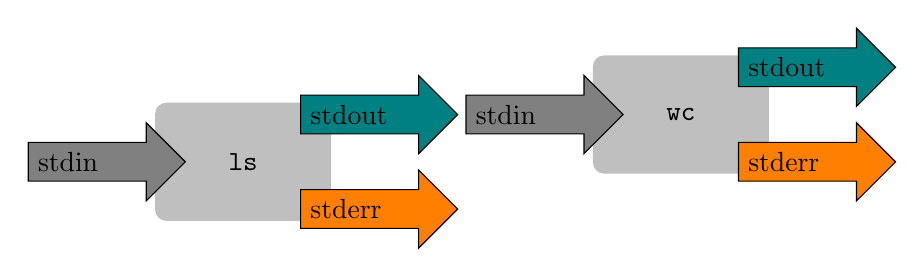
\begin{tikzpicture}
            \node [rounded corners, fill=gray!50, minimum height=15mm, text width=20mm, align=center]
                (ls)
                {\textbf{\texttt{ls}}};
            \node [draw, single arrow, fill=gray, anchor=east, text width=15mm] at ($(ls.west)+(4mm,0)$) {stdin};
            \node [draw, single arrow, fill=teal, anchor=west, text width=15mm] (stdout1) at ($(ls.east)+(-4mm,6mm)$) {stdout};
            \node [draw, single arrow, fill=orange, anchor=west, text width=15mm] at ($(ls.east)+(-4mm,-6mm)$) {stderr};

            \node [rounded corners, fill=gray!50, minimum height=15mm, text width=20mm, align=center, right=17mm of
                stdout1]
                (wc)
                {\textbf{\texttt{wc}}};
            \node [draw, single arrow, fill=gray, anchor=east, text width=15mm] at ($(wc.west)+(4mm,0)$) {stdin};
            \node [draw, single arrow, fill=teal, anchor=west, text width=15mm] at ($(wc.east)+(-4mm,6mm)$) {stdout};
            \node [draw, single arrow, fill=orange, anchor=west, text width=15mm] at ($(wc.east)+(-4mm,-6mm)$) {stderr};
        \end{tikzpicture}
    \end{center}
\end{frame}

%%%%%%%%%%%%%%%%%%%%%%%%%%%%%%%%%%%%%%%%%%%%%%%%%%%%%%%%%%%%%%%%%%%%%%%%%%%%%%%%%%%%%%%%%%%%%%%%%%%%

\begin{frame}[c,fragile]{\curtitle}
    Recall:
    \begin{shells}{\linewidth}
        \begin{shellout}
(*$\mathdollar$*) uniq -c duplicated_file.txt  (*$\dlsh$*) 
        \end{shellout}
        \begin{shellout}[stdout]
     22 bla
     28 blabla
      1 this line is not duplicatedbla
     21 bla
     28 blabla
        \end{shellout}
    \end{shells}
    Combining \command{sort} and \command{uniq}:
    \begin{shells}{\linewidth}
        \begin{shellout}
(*$\mathdollar$*) sort duplicated_file.txt | uniq -c (*$\dlsh$*) 
        \end{shellout}
        \begin{shellout}[stdout]
     43 bla
     56 blabla
      1 this line is not duplicatedbla
        \end{shellout}
    \end{shells}
\end{frame}

\begin{frame}[c,fragile]{\curtitle}
    What does this do and why?\bigskip

    \begin{shells}{\linewidth}
        \begin{shellout}
(*$\mathdollar$*) gunzip -c material.tar.gz | tar t (*$\dlsh$*) 
        \end{shellout}
    \end{shells}
\end{frame}

\end{document}
